\begin{frame}{Problem}
  This problem entails optimizing the placement of servers in a data center.

  \begin{itemize}
    \item The data center is modeled as a series of rows, each containing several
          slots in which servers can be placed.
    \item Certain slots may be unavailable due to other installations within the data
          center.
    \item Servers must be logically assigned to pools contributing with their (computing) capacity.
  \end{itemize}
\end{frame}

\begin{frame}{Example --- Data Center}
  \begin{figure}[h]
    \centering
    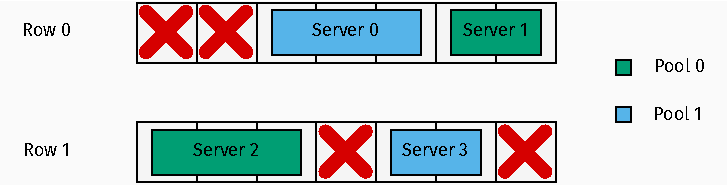
\includegraphics[width=0.9\textwidth,keepaspectratio]{../assets/dc/dc-slides.pdf}
    \caption{Example Data Center Layout}
  \end{figure}

  \begin{table}[ht]
    \centering
    \begin{tabular}{ccc}
      \toprule
      Server & Size & Capacity \\ \midrule
      1      & 3    & 2        \\
      2      & 2    & 5        \\
      3      & 3    & 10       \\
      4      & 2    & 3        \\ \bottomrule
    \end{tabular}
    \caption{Server Properties}
  \end{table}
\end{frame}

\begin{frame}{Guaranteed Capacity}
  The guaranteed capacity is a measure of the remaining computing capacity
  available for a given pool in the event that at most one arbitrary row of the
  data center becomes inoperable.

  \begin{equation*}
    \begin{aligned}
      gc_p(x)     = & \sum_{m=1}^\mathcal{M} \sum_{r=1}^\mathcal{R} \sum_{i \in \mathcal{I}^{r}} c_m \cdot x_{m,p,i} - \max_{r=1}^\mathcal{R} \sum_{m=1}^\mathcal{M} \sum_{i \in \mathcal{I}^r} c_m \cdot x_{m,p,i} \\
    \end{aligned}
  \end{equation*}
  Where,
  \begin{itemize}
    \item $\mathcal{M}$ is the number of servers.
    \item $\mathcal{R}$ is the number of rows.
    \item $\mathcal{I}^{r}$ is a set containing the segment IDs for a given row $r$.
    \item $c_{m}$ is the computing capacity of the server $m$.
    \item $x_{m, p, i}$ is a binary variable indicating whether the server,~$m$, is assigned (1) or not (0) to pool,~$p$, and segment~$i$.
  \end{itemize}
\end{frame}

\begin{frame}{Example --- Guaranteed Capacity}
  \begin{figure}[h]
    \centering
    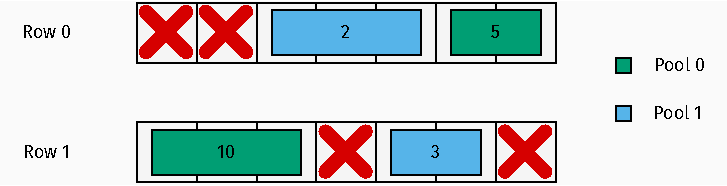
\includegraphics[width=0.9\textwidth,keepaspectratio]{../assets/dc/dc-slides-capacity.pdf}
    \caption{Example Data Center Layout (Capacities Only)}
  \end{figure}

  \begin{table}[ht]
    \centering
    \begin{tabular}{@{\extracolsep{4pt}}cccc}
      \toprule
      Pool & Row 1 & Row 2 & Guaranteed Capacity \\ \midrule
      1    & 5     & 10    & 5                   \\
      2    & 2     & 3     & 2                   \\
      \bottomrule
    \end{tabular}
    \caption{Guaranteed Capacities}
  \end{table}
\end{frame}

\begin{frame}{Problem Formulation}
  \begin{equation*}
    \begin{aligned}
      \max\ f(x)   & = \min_{p=1}^\mathcal{P}{gc_{p}(x)}                                                                                                \\
      \text{s.t. } & \sum_{p=1}^{\mathcal{P}} \sum_{r=1}^{\mathcal{R}} \sum_{i \in \mathcal{I}^{r}} x_{m,p,i} \le 1 & \forall\ m=1,\ldots,\mathcal{M}   \\
                   & \sum_{m=1}^{\mathcal{M}} \sum_{p=1}^{\mathcal{P}} \ell_m \cdot x_{m,p,i} \le \mathcal{L}_{i}   & \forall\  i=1,\ldots, \mathcal{I} \\
                   & x \in {\{0,1\}}^{\mathcal{M} \times \mathcal{P} \times \mathcal{R}}                                                                \\
    \end{aligned}
  \end{equation*}
  Where,
  \begin{itemize}
    \item $\mathcal{P}$ is the number of pools
    \item $\mathcal{I}$ is the number of segments
    \item $\mathcal{L}_{i}$ is the size of segment $i$
    \item $l_{m}$ is the size of the server $m$.
  \end{itemize}
\end{frame}

\begin{frame}{Example --- Objective}
  \begin{figure}[h]
    \centering
    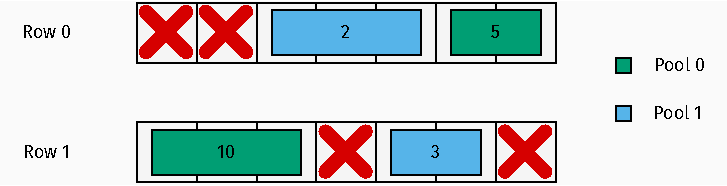
\includegraphics[width=0.9\textwidth,keepaspectratio]{../assets/dc/dc-slides-capacity.pdf}
  \end{figure}

  \begin{table}[ht]
    \centering
    \begin{tabular}{@{\extracolsep{4pt}}ccccc}
      \toprule
      Pool & Row 1 & Row 2 & Guaranteed Capacity & \textbf{$f(x)$}              \\ \midrule
      1    & 5     & 10    & 5                   &                              \\
      2    & 2     & 3     & 2                   & \multirow{-2}{*}{\textbf{2}} \\
      \bottomrule
    \end{tabular}
    \caption{Guaranteed Capacities \& Objective Value}
  \end{table}
\end{frame}

\begin{frame}{Modeling --- Problem, Solution and Component}
  The~\alert{problem} is characterized by the set of available servers, along with
  their respective sizes and capacities, the number of resource pools to be
  created, and the set of segments.

  A~\alert{solution} is characterized by a collection of server assignments to
  pools and segments.

  A~\alert{component} is characterized by a tuple containing a server
  a pool and a segment or just a server (indicating that is forbidden from being assigned).
\end{frame}

\begin{frame}{Modeling --- Construction Rules}
  Three component enumeration strategies were considered:

  \begin{itemize}
    \item \textbf{Standard:} Enumerate all feasible combinations of assignments
          of servers to pools and segments.
    \item \textbf{Sequential:} For one server at a time enumerate all feasible
          assignments to pools and segments.
    \item \textbf{Heuristic:} Select an order for the servers pools and segments
          and enumerate all possible assignments following that order.
  \end{itemize}

  Notably, the component associated with the action of forbidding a server is
  always feasible in any enumeration.
\end{frame}

\begin{frame}{Modeling --- Upper Bound}
  The first upper bound devised for this problem is calculated in through the following steps:
  \begin{enumerate}
    \item \textbf{Relax Segments Constraint:} Remove one row and treat the total available slots in all other rows as a knapsack.

    \item \textbf{Optimize Computing Capacity:} Find the best computing capacity achievable by placing servers in this knapsack.

    \item \textbf{Estimate Guaranteed Capacity:} Divide the capacity by the total number of pools for an optimistic guaranteed capacity estimate.

    \item \textbf{Apply Correction:} If this estimate exceeds the capacity already assigned to any pool.

    \item \textbf{Iterate and Determine Upper Bound:} Repeat these steps for all
          remaining rows, and the upper bound is the minimum value for the guaranteed
          capacity obtained through this process.
  \end{enumerate}

\end{frame}

\begin{frame}{Modeling --- Upper Bound}
  The second upper bound is a slight variation of the previous bound where
  instead of selecting the minimum value in each iteration, a~\textbf{vector containing
    the minimum value for each pool} is kept.

  The~\textbf{upper bound} value is given by this~\textbf{vector sorted in increasing order}.

  Notably, the objective function must be updated where a sorted vector
  containing all the guaranteed capacities serves as the objective value.

  \begin{table}[ht]
    \centering
    \begin{tabular}{@{\extracolsep{4pt}}ccccc}
      \toprule
      Pool & Row 1 & Row 2 & Guaranteed Capacity & \textbf{$f(x)$}                   \\ \midrule
      1    & 5     & 10    & 5                   &                                   \\
      2    & 2     & 3     & 2                   & \multirow{-2}{*}{\textbf{(2, 5)}} \\
      \bottomrule
    \end{tabular}
    \caption{Guaranteed Capacities \& Objective Value}
  \end{table}
\end{frame}

\begin{frame}{Modeling --- Local Moves}
  The~\alert{local moves} considered for this problem are as follows:

  \begin{enumerate}
    \item \textbf{Assigning a server} to a pool and segment if there is an available one.
    \item \textbf{Removing a server} from a segment.
    \item \textbf{Changing the segment} to which a particular server is allocated.
    \item \textbf{Changing the pool} to which a server is allocated, moving it to a different pool.
    \item \textbf{Swapping the pools} of two assigned servers.
    \item \textbf{Swapping the segments} of two assigned servers.
  \end{enumerate}
\end{frame}

\begin{frame}{Results}
  We were able to achieve a objective value of~\alert{386} on the single instance that was
  available through a~\textbf{simple constructive meta-heuristic}.

  Then an~\textbf{Iterated Local Search} meta-heuristic was applied to further
  exploit this solution. The objective value obtained through this process
  was~\alert{410}, which would have placed us in~\textbf{1st place} on the
  competition leaderboard.

  Notably, the best known objective value is~\textbf{408}.
\end{frame}